% !TeX spellcheck = pl_PL

\rozdzial

%%%%%%%%%%%%%%%%%%%%%%%%%%%%%%%%%%%%%%%%%%%%%%%%%%%%%%%%%%%%%%%%%%%%%%%
\section{Logowanie i zarządzanie użytkownikami}

\subsection{Logowanie}

Program uruchamia się za pomocą dwukrotnego kliknięcia na ikonę DotBase.exe.
Po uruchomieniu aplikacji pojawia się okno logowania (rys. \ref{oknoLogowania}).

W prawym dolnym rogu znajduje się aktualna wersja programu.

\begin{figure}[htb]
	\centering
	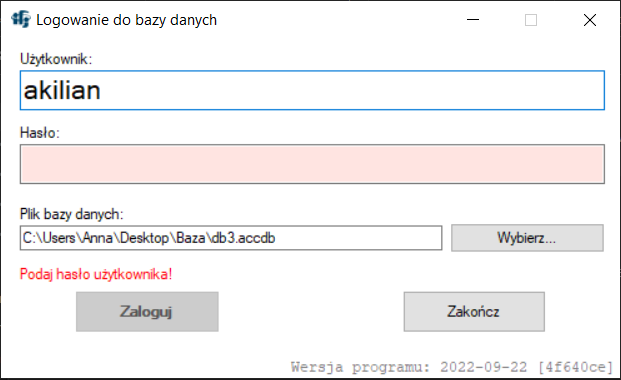
\includegraphics{obrazki/Logowanie/logowanie.png}
	\caption{Okno logowania}
	\label{oknoLogowania}
\end{figure}

W pierwszej kolejności należy podać bezwzględną ścieżkę do pliku bazy danych, na której zamierza się pracować. Można również wybrać plik bazy, korzystając z przycisku \textbf{"Wybierz..."}, który otwiera okno eksploratora plików Windows. 

\textbf{TIP:} Program zapamiętuje ostatnią podaną ścieżkę i automatycznie wpisuje ją przy kolejnym uruchomieniu.

Jeżeli ścieżka do bazy danych jest wybrana należy wpisać przydzielony login i hasło i nacisnąć przycisk \textbf{"Zaloguj"}.
Jeżeli mamy uprawnienia administratora, to po wpisaniu poprawnego loginu i hasła pojawia się dodatkowy przycisk \textbf{"Administracja"} (rys. \ref{oknoLogowaniaAdmina}). Przycisk ten przenosi nas do części programu związanej z zarządzaniem hasłami i dostępem użytkowników (patrz \ref{}).

\begin{figure}[htb]
	\centering
	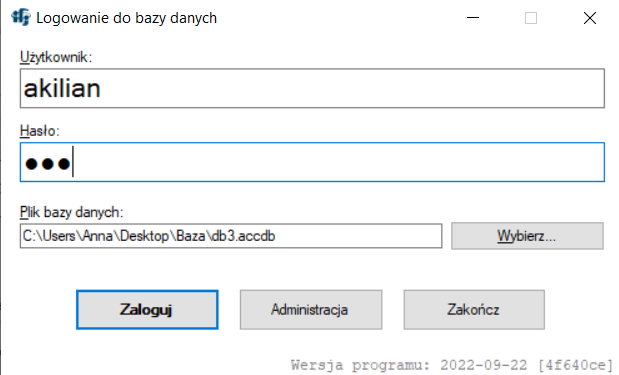
\includegraphics{obrazki/Logowanie/logowanie_administracja.png}
	\caption{Okno logowania administratora}
	\label{oknoLogowaniaAdmina}
\end{figure}

\begin{figure}[htb]
	\centering
	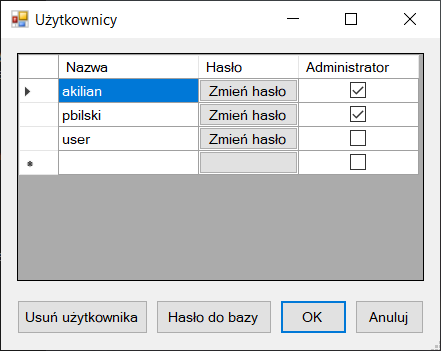
\includegraphics{obrazki/Logowanie/administracja.png}
	\caption{Okno zarządzania dostępem użytkowników}
	\label{administracja}
\end{figure}

\begin{figure}[htb]
	\centering
	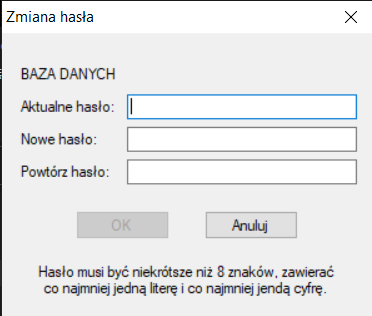
\includegraphics{obrazki/Logowanie/zmiana_hasla_bazy.png}
	\caption{Okno zmiany hasła do bazy danych}
	\label{zmianaHaslaBazy}
\end{figure}

\begin{figure}[htb]
	\centering
	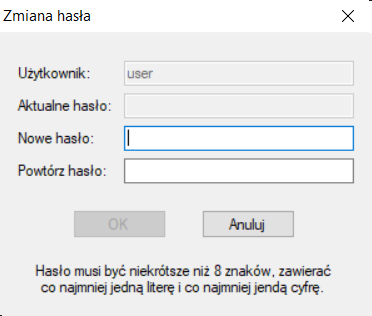
\includegraphics{obrazki/Logowanie/zmiana_hasla_uzytkownika.png}
	\caption{Okno zmiany hasła użytkownika}
	\label{zmianaHaslaUzytkownika}
\end{figure}
